% !TEX program = xelatex

\documentclass[10pt,a4paper]{article}
\usepackage[top = 1.5cm, bottom = 1.5cm, left = 1.5cm, right = 1.5cm]{geometry}
\usepackage{wrapfig}
\usepackage{float}

\usepackage{titling}
\usepackage[czech]{babel}
\usepackage{graphicx}
\usepackage{lmodern}
\usepackage{hyperref}
\usepackage{setspace}
\usepackage{csvsimple}

\usepackage{amsmath}
\usepackage{amssymb}
\usepackage{gensymb}
\usepackage{mathtools}
\usepackage{units}
\usepackage{bm}
\delimitershortfall=-1pt



% redefine \sqrt
\usepackage{letltxmacro}
\makeatletter
\let\oldr@@t\r@@t
\def\r@@t#1#2{%
\setbox0=\hbox{$\oldr@@t#1{#2\,}$}\dimen0=\ht0
\advance\dimen0-0.2\ht0
\setbox2=\hbox{\vrule height\ht0 depth -\dimen0}%
{\box0\lower0.4pt\box2}}
\LetLtxMacro{\oldsqrt}{\sqrt}
\renewcommand*{\sqrt}[2][\ ]{\oldsqrt[#1]{#2\,}\,}
\makeatother



\DeclarePairedDelimiter\ceil{\lceil}{\rceil}
\DeclarePairedDelimiter\floor{\lfloor}{\rfloor}

\def\ph{\phantom}
\def\vph{\vphantom}
\def\hph{\hphantom}
\def\rzw{\mathrlap}
\def\lzw{\mathllap}
\def\czw{\mathclap}

\def\?{\mathit{?}}

\def\+{+\!\!}
\def\-{-\!\!}

\newcommand{\comm}[2]{\left[ #1, #2 \right]}
\newcommand{\const}[1]{\text{#1}}
\newcommand{\norm}[1]{\left\lVert#1\right\rVert}

\newcommand{\mat}[1]{
    \begin{pmatrix}
        #1
    \end{pmatrix}
}

\newcommand{\mata}[2]{
    \left(
    \begin{array}{@{}#1@{}}
        #2
    \end{array}
    \right)
}

\newcommand{\smat}[2][1]{
    \scalebox{#1}{$\mat{#2}$}
}

\newcommand{\tg}{\operatorname{tg}}
\newcommand{\cotg}{\operatorname{cotg}}
\newcommand{\Res}{\operatorname{Res}}
\renewcommand{\Re}{\operatorname{Re}}

\renewcommand{\d}[1]{\;\const{d}#1}
\newcommand{\dd}[2]{\frac{\const{d} #1}{\const{d} #2} \;}
\newcommand{\pd}[2]{\frac{\partial  #1}{\partial  #2} \;}

\newcommand{\bra}[1]{\left< #1 \right|}
\newcommand{\ket}[1]{\left| #1 \right>}
\newcommand{\braket}[2]{\left< #1 \middle| #2 \right>}

\newcommand{\bhat}[1]{\hat{\bm{#1}}}

\newcommand{\e}[1]{\const{e}^{#1}}
\renewcommand{\i}{\const{i}}

\newcommand{\concurrent}{{\upharpoonleft\!\upharpoonright}}
\newcommand{\countercurrent}{{\upharpoonleft\!\downharpoonright}}

\newcommand{\textmath}[2]{\texorpdfstring{$#2$}{#1}}

\begin{document}

\title{Matematika pro Fyziky 2: DÚ 3}
\author{Michal Grňo}
\date{\today}

\maketitle

\section{Příklad 5}
\subsection{Zadání}
\begin{equation*}
    I = \int_0^{+\infty}\frac{\cosh ax}{\cosh \pi x} \d{x},
    \hspace{2em}
    |a|<\pi, \; a \in \mathbb{R}
\end{equation*}

\subsection{Řešení}
Jde o sudou funkci, proto můžeme integrál rozšířit na interval $(-\infty, \infty)$:
\begin{equation*}
    I = \frac{1}{2} \int_{-\infty}^{+\infty}\frac{\cosh ax}{\cosh \pi x} \d{x}.
\end{equation*}
Výraz si přepíšeme pomocí vzorce $\cosh x = \e{x} + \e{-x}$ a přejdeme do $\mathbb{C}$:
\begin{equation*}
    I = \frac{1}{2} \int_{-\infty}^{+\infty}\frac{\e{az} + \e{-az}}{\e{\pi z} + \e{-\pi z}} \d{z}
    = \frac{1}{2} \Big( \underbrace{\int_{-\infty}^{+\infty}\frac{\e{az}}{\e{\pi z} + \e{-\pi z}} \d{z}}_{I_1} + \underbrace{\int_{-\infty}^{+\infty}\frac{\e{-az}}{\e{\pi z} + \e{-\pi z}} \d{z}}_{I_2} \Big).
\end{equation*}
\begin{equation*}
    f_1(z) = \frac{\e{az}}{\e{\pi z} + \e{-\pi z}},
    \hspace{2em}
    f_2(z) = \frac{\e{-az}}{\e{\pi z} + \e{-\pi z}}.
\end{equation*}

Funkce mají singularity v bodech:
\begin{equation*}
    \e{\pi z} + \e{-\pi z} = 0 \; \Leftrightarrow \; z = \i (n + \frac{1}{2}).
\end{equation*}

Integrál $I$ vypočteme pomocí křivkového integrálu v komplexní rovině:
\begin{figure}[H]
    \centering
    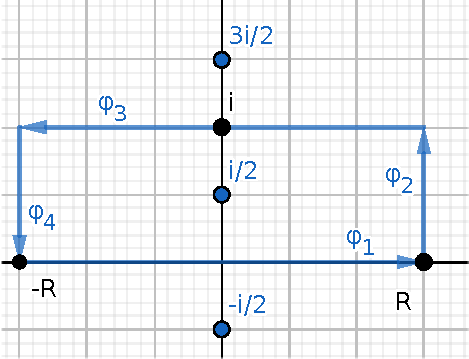
\includegraphics[width=0.4\textwidth]{du3u1param.pdf}
\end{figure}
\begin{equation*}
    \varphi = \varphi_1 \oplus \varphi_2 \oplus \varphi_3 \oplus \varphi_4
\end{equation*}
\begin{align*}
    \varphi_1 &= t \mapsto Rt, \; t \in [-1, 1], \\
    \varphi_2 &= t \mapsto R + \i t, \; t \in [0, 1], \\
    \varphi_3 &= t \mapsto -Rt, \; t \in [-1, 1] \\
    \varphi_4 &= t \mapsto -R + \i(1-t), \; t \in [0, 1]
\end{align*}
\begin{align*}
    \int_\varphi f_1 \d{z} = 2\pi\i \Res_{\nicefrac{\i}{2}} f_1,
    \hspace{2em}
    \int_\varphi f_2 \d{z} = 2\pi\i \Res_{\nicefrac{\i}{2}} f_2,
\end{align*}
\begin{equation*}
    \int_{\varphi_1} f_1 \d{z} = \e{\i a} \int_{\varphi_3} f_1 \d{z},
    \hspace{2em}
    \int_{\varphi_1} f_2 \d{z} = \e{-\i a} \int_{\varphi_3} f_2 \d{z}.
\end{equation*}

Budeme zkoumat vývoj při $R \to \infty$. Vidíme, že integrály přes $\varphi_2$ a $\varphi_4$ vymizí:
\begin{align*}
    z \to +\infty: \; &\frac{\e{az} + \e{-az}}{\e{\pi z} + \e{-\pi z}}
    \sim \e{(|a|-\pi)z} \to 0
    \\
    z \to -\infty: \; &\frac{\e{az} + \e{-az}}{\e{\pi z} + \e{-\pi z}}
    \sim \e{-(|a|-\pi)z} \to 0
\end{align*}
Naopak integrály přes $\varphi_1$ a $\varphi_3$ zkonvergují k násobku $I$. Vypočteme nyní rezidua.
\begin{equation*}
    \Res_{\nicefrac{\i}{2}} f_1
    = \Res_{\nicefrac{\i}{2}} \frac{\e{az}}{\e{\pi z} + \e{-\pi z}}
    = \frac{\e{\i a/2}}{\pi\e{\i\pi/2} + \pi\e{-\i\pi/2}}
    = \frac{1}{2\pi\i} \e{\i a/2}
\end{equation*}
\begin{equation*}
    \Res_{\nicefrac{\i}{2}} f_2
    = \Res_{\nicefrac{\i}{2}} \frac{\e{-az}}{\e{\pi z} + \e{-\pi z}}
    = \frac{\e{-\i a/2}}{\pi\e{\i\pi/2} + \pi\e{-\i\pi/2}}
    = \frac{1}{2\pi\i} \e{-\i a/2}
\end{equation*}
Nyní už víme všechno potřebné pro výpočet výsledku:
\begin{align*}
    \int_\varphi f_1 \d{z}
    &= \int_{\varphi_1} f_1 \d{z} + \int_{\varphi_3} f_1 \d{z}
    &
    \int_\varphi f_2 \d{z}
    &= \int_{\varphi_1} f_2 \d{z} + \int_{\varphi_3} f_2 \d{z}
    \\
    2\pi\i \Res_{\nicefrac{\i}{2}} f_1
    &= (1+\e{\i a}) \int_{\varphi_1} f_1 \d{z}
    &
    2\pi\i \Res_{\nicefrac{\i}{2}} f_2
    &= (1+\e{-\i a}) \int_{\varphi_1} f_2 \d{z}
    \\
    \int_{\varphi_1} f_1 \d{z}
    &= \frac{\e{\i a}}{1+\e{\i a}}
    &
    \int_{\varphi_1} f_2 \d{z}
    &= \frac{\e{-\i a}}{1+\e{-\i a}}
\end{align*}
\begin{equation*}
    2I = 2I_1 + 2I_2
    = \int_{\varphi_1} f_1 \d{z} + \int_{\varphi_1} f_2 \d{z}
    = \frac{\e{\i a}}{1+\e{\i a}} + \frac{\e{-\i a}}{1+\e{-\i a}}
    = \frac{2\e{\i a/2} + 2\e{-\i a/2}}{2 + \e{\i a} + \e{-\i a}}
    = \frac{1}{\cos \frac{a}{2}}
\end{equation*}
\bigskip
\begin{equation*}
    \int_0^{+\infty}\frac{\cosh ax}{\cosh \pi x} \d{x} = \frac{1}{2 \cos \frac{a}{2}}.
\end{equation*}

\pagebreak

\section{Příklad 13}
\subsection{Zadání}
\begin{equation*}
    I = \int_0^1 \frac{x^{1-p} (1-x)^p}{x^2+1} \d{x},
    \hspace{2em}
    p \in (-1, 2)
\end{equation*}

\end{document}